\subsection{Technical overview}\label{sec:approach}\label{sec:overview}\label{ov:structure}

Rather than extending the fooling-set argument in~\S\ref{sec:natural-approaches}, we abandon witness crossing and embeddings altogether. Instead, we compare a reference structure with its local modifications using exact predictions that commute with complement.

\smallskip
\customparagB{Our technique: The two-witness property.}
We use a complete undirected graph $\mathbb{G} = (V,\chi)$ whose edges are colored by the $2^k$ subsets of $[k]$.
We write $\chi(u,v)=\chi(v,u)$ for the color of the edge between distinct vertices $u$ and $v$,
and use $\lambda,\mu,\nu$ for colors.
The key property of $\mathbb{G}$ is the \defn{two-witness property}: for all distinct
$u,v\in V$ and all colors $\mu,\nu$,\nakamura{図の $u$--$v$ の点線の意図が不明です（$z$--$z'$にないのはなぜ）}
\[
\text{at least two vertices $z\notin\{u,v\}$ satisfy $\chi(u,z)=\mu$ and
 $\chi(z,v)=\nu$.}
 \qquad
 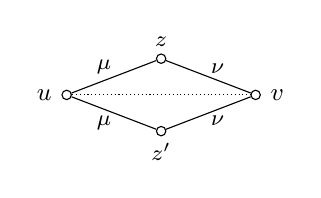
\begin{tikzpicture}[baseline={([yshift=-0.55ex]u.center)},
   every node/.style={font=\footnotesize},vtx/.style={circle,draw,inner sep=1.2pt}]
 \node[vtx,label={[font=\small]left:$u$}] (u) at (0,0) {};
 \node[vtx,label={[font=\small]right:$v$}] (v) at (2.4,0) {};
 \node[vtx,label={[label distance=-1pt]above:$z$}] (z) at (1.2,0.46) {};
 \node[vtx,label={[label distance=-1pt]below:$z'$}] (z2) at (1.2,-0.46) {};
 \draw (u) -- node[above left=-2.5pt] {$\mu$} (z);
 \draw (z) -- node[above right=-2.5pt] {$\nu$} (v);
 \draw (u) -- node[below left=-2.5pt] {$\mu$} (z2);
 \draw (z2) -- node[below right=-2.5pt] {$\nu$} (v);
 \draw[densely dotted] (u) -- (v);
 \end{tikzpicture}
\]
We call such vertices $z$ \defn{witnesses}.
A coloring with this property exists whenever
$|V|\ge n_0(2^k)$, where
$n_0(N)\coloneqq\lceil12N^2\ln(2N)\rceil+3$, since a uniformly random
coloring has it with positive probability
(Lemma~\ref{lem:palette}). These colorings go back to Jipsen, Maddux, and
Tuza~\citep{jipsen-maddux-tuza1995}.

\paragraph{Roadmap.}
In \S\ref{ov:fold}, we construct $2^k$ folds of the reference structure $\mathcal M_0$, each changing the answer of $G_k$ at an unchanged edge.
%
In \S\ref{ov:types}, we show that every circuit gate on $\mathcal M_0$ is constant on each edge-color class and on the diagonal. This allows us to define predictions under each fold.
Boolean operations, including complement, and converse preserve these predictions; only composition can violate them.
%
In \S\ref{ov:twocolors}, we show that, thanks to the two-witness property, each composition can violate the prediction for at most two folds. Since every fold must be detected, any circuit for $G_k$ requires at least $2^{k-1}$ compositions, even with sharing.
\nakamura{violate / detect / notice は重複？（notice は後で定義がある）}

\subsubsection{Folding the reference structure}\label{ov:outline}\label{ov:fold}

We use the reference coloring $\chi$ to define an input structure $\mathcal M_0$ for $G_k$.
On an edge of color $\mu$, we interpret $P_i$ as true exactly when $i\in\mu$, and $Q_i$ exactly when $i\notin\mu$. No input relation holds on loops, which carry the separate label $\id$.
Consequently, a read edge of color $\mu$ accepts exactly witness edges of color $\mu^c$: for distinct $u,v$,
\[
\mathcal M_0 \models G_k(u,v)\iff
\exists z \notin \set{u, v}.\ \chi(u,z)=\chi(u,v)^c.
\]
By the two-witness property, every vertex
has edges of every color, so $G_k$ holds
at every non-loop pair of $\mathcal M_0$.

Fix a vertex $\hub \in V$, the \defn{hub}, and for each color $\mu$ choose $v_\mu$ with $\chi(\hbar,v_\mu)=\mu$.
\nakamura{$\hbar$, $h$, $\hub$ が混在}
%
For each color $\lambda$, let $\chi_\lambda$ be obtained from $\chi$ by recoloring every $\lambda$-colored edge incident to $\hub$ as $\lambda^c$, leaving all other edges unchanged.
Let $\mathcal M_\lambda$ be the input structure induced by $\chi_\lambda$ in the same way as $\mathcal M_0$.
In $\mathcal M_\lambda$, the hub has no edge of color $\lambda$, but the read edge $(\hub,v_{\lambda^c})$ remains unchanged (Figure~\ref{fig:fold}).

\begin{figure}[H]
\begin{minipage}[c]{0.27\linewidth}
\setlength{\abovecaptionskip}{0pt}
\caption[The fold of $\lambda$]{\raggedright The fold of $\lambda$. Only edges at the hub $\hub$ are drawn.}
\label{fig:fold}
\end{minipage}\hfill
\begin{minipage}[c]{0.71\linewidth}
\centering
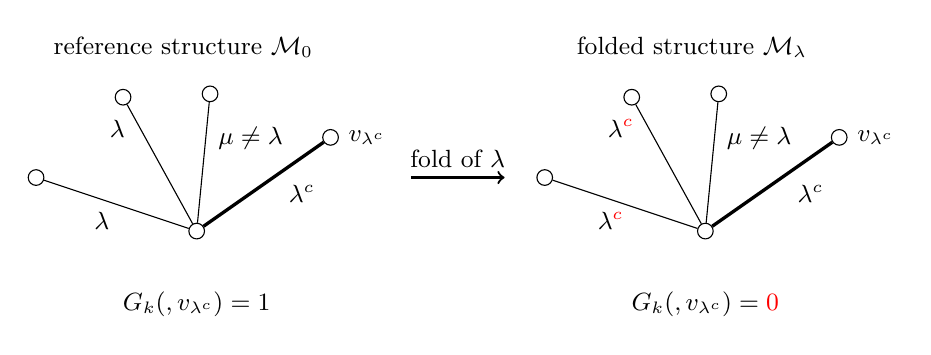
\begin{tikzpicture}[scale=0.85,every node/.style={font=\small},
  vtx/.style={circle,draw,inner sep=2pt}]
\foreach \xs/\col/\val/\name in
  {0/\lambda/1/{reference structure $\mathcal M_0$},
   7.6/\lambda^{\color{red}c}/{\color{red}0}/{folded structure $\mathcal M_\lambda$}}{
\begin{scope}[xshift=\xs cm]
\node at (-0.2,2.75) {\name};
\node[vtx,label={[label distance=2pt]below:$\hub$}] (h) at (0,0) {};
\node[vtx] (a1) at (-2.4,0.8) {};
\node[vtx] (a2) at (-1.1,2.0) {};
\node[vtx] (x) at (0.2,2.05) {};
\node[vtx,label=right:$v_{\lambda^c}$] (v) at (2.0,1.4) {};
\draw (h)--node[below=1pt,pos=0.6] {$\col$} (a1);
\draw (h)--node[left=2pt,pos=0.8] {$\col$} (a2);
\draw (h)--node[right=1pt,pos=0.7] {$\mu\ne\lambda$} (x);
\draw[very thick] (h)--node[below right=0pt,pos=0.62] {$\lambda^c$} (v);
\node at (0,-1.1) {$G_k(\hub,v_{\lambda^c})=\val$};
\end{scope}}
\draw[->,thick] (3.2,0.8)--node[above]{fold of $\lambda$} (4.6,0.8);
\end{tikzpicture}
\end{minipage}
\end{figure}

The read edge $(\hub,v_{\lambda^c})$ requires a $\lambda$-colored edge at $\hub$; the fold removes all such edges. 
\nakamura{辺は削除ではなく、ラベルの反転 (flip)、あるいはラベルの変更か (Fig~\ref{fig:prediction}周辺も同様)}
Hence
\[
\chi_\lambda(\hbar,v_{\lambda^c})
 =\chi(\hbar,v_{\lambda^c})=\lambda^c,\ 
\mathcal M_0\models G_k(\hbar,v_{\lambda^c}),\ 
\mathcal M_\lambda\not\models G_k(\hbar,v_{\lambda^c}).
\]
We call $(\mathcal M_0,\mathcal M_\lambda,(\hub,v_{\lambda^c}))$ the \defn{test} for $\lambda$.
Thus $G_k$ yields $2^k$ tests, one for each color.

\if0
Fix, for each color $\mu$, a vertex $v_\mu$ with $\chi(\hub,v_\mu)=\mu$.
The read edge $(\hub,v_{\lambda^c})$, which the fold of $\lambda$ does not
recolor since $\lambda^c\ne\lambda$, accepts exactly the witness edges of
color $\lambda$. So $G_k(\hub,v_{\lambda^c})$ holds exactly when $\hub$
has an edge of color $\lambda$. Writing $\sem\varphi{\mathcal M}$ also for
the relation that a gate $\varphi$ computes on $\mathcal M$, with value
$\sem\varphi{\mathcal M}(u,v)\in\{0,1\}$ at a pair $(u,v)$, we therefore
get
\[
 \mathcal M_0\xrightarrow{\ \text{fold }\lambda\ }\mathcal M_\lambda
 \quad(\lambda\subseteq[k]),\qquad
 \sem{G_k}{\mathcal M_0}(\hub,v_{\lambda^c})=1\ne0
 =\sem{G_k}{\mathcal M_\lambda}(\hub,v_{\lambda^c}).
\]
We call $\mathcal M_0$, $\mathcal M_\lambda$, and the read edge
$(\hub,v_{\lambda^c})$ the \defn{test} for $\lambda$. So for every color
$\lambda$, every circuit computing $G_k$ has different outputs at the read
edge on $\mathcal M_0$ and on $\mathcal M_\lambda$, although the fold does
not recolor this edge.
\fi


\subsubsection{Circuits see only colors}\label{ov:types}

\paragraph{Color-determined relations.}
A relation $X\subseteq V^2$ is
\defn{color-determined} if
$\chi(u,v)=\chi(u',v') \implies X(u,v)=X(u',v')$ holds.
Here loops carry the separate label $\id$.
Equivalently, $X$ is a union of edge-color
classes, possibly together with the diagonal.
Write $X[\mu]$ for its common value on edges
of color $\mu$, $X[\id]$ for its value on
loops.

Every gate of an arbitrary \CoR\ circuit computes a color-determined relation on $\mathcal M_0$ (Lemma~\ref{lem:tables}).
We can prove this by induction on the
circuit gates. Input relations and constants are
color-determined, while Boolean operations and
converse preserve this property.
The only nontrivial step is composition $X;Y$.

For distinct $u,v$, the two-witness property realizes every pair of colors $\mu,\nu$ along a path $u\xrightarrow{\mu}z\xrightarrow{\nu}v$ with $z\notin\set{u,v}$.
%
The case $z\in\set{u,v}$ depends only on $\chi(u,v)$ and the diagonal values of $X,Y$.
Hence $(X;Y)(u,v)$ depends only on $\chi(u,v)$.
For a loop $(u,u)$, both edges of a path $u-z-u$ have the same color, and every color occurs at every vertex. 
Together with the case $z=u$, this makes $(X;Y)(u,u)$ independent of $u$, completing the induction.


\paragraph{Predicting and noticing a fold.}
A color-determined relation $X$ assigns a value $X[\mu]$ to each color $\mu$.
To predict the effect of a fold, we keep these values fixed and read them at the new edge colors:
\[
\defn{(Prediction)}\quad
X^{(\lambda)}(u,v):=X[\chi_\lambda(u,v)].
\]
Thus a recolored edge reads $X[\lambda^c]$ rather than $X[\lambda]$; all other pairs retain their values.
%
This predicts what a gate would compute if its color-dependent behavior on $\mathcal M_0$ remained unchanged after the fold;
its actual value on $\mathcal M_\lambda$ may differ.

Input relations and constants behave exactly as predicted.
Moreover, Boolean operations and converse commute with prediction
(Proposition~\ref{prop:prediction-commutation}); in particular,
$\overline{X^{(\lambda)}}=(\overline X)^{(\lambda)}$.
Unlike the preservation under embeddings~\eqref{eq:mono} in \S\ref{sec:natural-approaches},
this equality survives unrestricted complement.

Figure~\ref{fig:prediction} compares three operations for any two
distinct colors $\lambda,\mu$: $X$ selects the $\lambda$-colored
edges, and $Y$ the $\mu$-colored edges (both exclude loops).
The thick edge $e=(\hub,v_\mu)$ is unchanged by the fold of
$\lambda$, which removes all $X^{(\lambda)}$-edges at $\hub$.\nakamura{Fig.~\ref{fig:prediction} の表が読めない気がします。列見出しをもう少しちゃんと書くか、caption か本文に説明が欲しいです。
また、Fig.~\ref{fig:prediction} は Fig.~\ref{fig:fold} とほぼ同じにもみえます（あと、塗り替えた辺が Fig.~\ref{fig:prediction} では破線、Fig.~\ref{fig:fold} では実線で、整合性が取れていない）}

\begin{figure}[H]
  \centering
  \begin{minipage}[c]{0.58\linewidth}
    \centering
\begin{tikzpicture}[
      >=Latex,
      vertex/.style={circle,draw,fill=white,inner sep=0pt,minimum size=3.2pt},
      edge/.style={line width=.5pt},
      read/.style={line width=1.05pt},
      folded/.style={draw=red!65!black,densely dashed,line width=.75pt},
      every node/.style={font=\scriptsize},
    ]
      % These four vertices show two of the witnesses; the full arena
      % contains further vertices and satisfies the two-witness property.
      \coordinate (h0) at (0,0);
      \coordinate (v0) at (2.65,0);
      \coordinate (z0) at (1.325,0.98);
      \coordinate (w0) at (1.325,-0.98);
      \draw[read] (h0)--node[below,pos=.54] {$\mu$} (v0);
      \draw[edge] (h0)--node[above left] {$\lambda$} (z0);
      \draw[edge] (h0)--node[below left] {$\lambda$} (w0);
      \draw[edge] (z0)--node[above right] {$\mu$} (v0);
      \draw[edge] (w0)--node[below right] {$\mu$} (v0);
      \node[vertex,label=left:{$\hub$}] at (h0) {};
      \node[vertex,label=right:{$v_\mu$}] at (v0) {};
      \node[vertex,label=above:{$z$}] at (z0) {};
      \node[vertex,label=below:{$z'$}] at (w0) {};
      \node[font=\small] at (.1, 1.2) {$\mathcal M_0$};
      \draw[-{Latex[length=2mm]},line width=.7pt]
        (3.4,0)--node[above] {fold $\lambda$} (4.85,0);
      \begin{scope}[xshift=5.30cm]
        \coordinate (h1) at (0,0);
        \coordinate (v1) at (2.65,0);
        \coordinate (z1) at (1.325,0.98);
        \coordinate (w1) at (1.325,-0.98);
        \draw[read] (h1)--node[below,pos=.54] {$\mu$} (v1);
        \draw[folded] (h1)--node[above left,black] {$\lambda^c$} (z1);
        \draw[folded] (h1)--node[below left,black] {$\lambda^c$} (w1);
        \draw[edge] (z1)--node[above right] {$\mu$} (v1);
        \draw[edge] (w1)--node[below right] {$\mu$} (v1);
        \node[vertex,label=left:{$\hub$}] at (h1) {};
        \node[vertex,label=right:{$v_\mu$}] at (v1) {};
        \node[vertex,label=above:{$z$}] at (z1) {};
        \node[vertex,label=below:{$z'$}] at (w1) {};
        \node[font=\small] at (.1, 1.2) {$\mathcal M_\lambda$};
      \end{scope}
    \end{tikzpicture}
  \end{minipage}\hfill%
  \begin{minipage}[c]{0.40\linewidth}
    \centering
    {\footnotesize
    \renewcommand{\arraystretch}{1.16}%
    \begin{tabular}{@{}lccc@{}}
      \toprule
      Operation & Predicted & Actual & Notice? \\
      \midrule
      $X;Y$         & $1$ & $0$ & Yes \\
      $X\cup Y$     & $1$ & $1$ & No \\
      $\overline X$ & $1$ & $1$ & No \\
      \bottomrule
    \end{tabular}}
  \end{minipage}
  \caption{At $e=(\hub,v_\mu)$, only composition notices the fold of $\lambda$.
    Only two witness paths are shown; all $\lambda$-edges at $\hub$ are recolored to $\lambda^c$.}
  \label{fig:prediction}
\end{figure}

\if0
An operation \defn{notices} a fold at given color-determined
operands if applying it after prediction differs from predicting its
result. In Figure~\ref{fig:prediction}, composition notices the fold:
$X^{(\lambda)};Y^{(\lambda)}\ne(X;Y)^{(\lambda)}$.
Union and complement do not notice it; indeed, Proposition~\ref{prop:prediction-commutation}
shows that no Boolean operation or converse can ever notice a fold.
\fi

An operation \defn{notices} a fold at given
color-determined operands if applying it to
their predictions differs from predicting
its result. In Figure~\ref{fig:prediction}, composition notices
the fold at $e$, since
\[
  e\notin\bigl(X^{(\lambda)};Y^{(\lambda)}\bigr)
  \quad \text{and} \quad
  e\in(X;Y)^{(\lambda)}.
\]
By contrast, union and complement do not
notice the fold. More generally, no Boolean
operation or converse can notice any fold
(Proposition~\ref{prop:prediction-commutation}).

Every fold must be noticed by some composition gate.
Let $C$ be a \CoR\ circuit such that $C\equiv G_k$.
If no composition gate notices the fold of $\lambda$,
then, since $(\hub,v_{\lambda^c})$ is unchanged,
Lemma~\ref{lem:unnoticed} gives
\[
  \mathcal M_0\models C(\hub,v_{\lambda^c})
  \quad\Longleftrightarrow\quad
  \mathcal M_\lambda\models C(\hub,v_{\lambda^c}).
\]
This contradicts $C\equiv G_k$, since
$\mathcal M_0\models G_k(\hub,v_{\lambda^c})$
but $\mathcal M_\lambda\not\models G_k(\hub,v_{\lambda^c})$.

\if0
Every fold must be noticed by some composition gate.
Now let $C$ be any circuit computing $G_k$.
If no composition gate notices the fold of
$\lambda$, Lemma~\ref{lem:unnoticed} implies that the output
on $\mathcal M_\lambda$ is the prediction
of the output on $\mathcal M_0$.
Since the test edge $e_\lambda=(\hub,v_{\lambda^c})$ is unchanged,
\[
\sem{C}{\mathcal M_\lambda}(e_\lambda)
=
\bigl(\sem{C}{\mathcal M_0}
\bigr)^{(\lambda)}(e_\lambda)
=
\sem{C}{\mathcal M_0}(e_\lambda),
\]
contradicting the test for $\lambda$, whose outputs are $0$ on $\mathcal M_{\lambda}$ and $1$ on $\mathcal M_0$.
\fi


\subsubsection{Each composition notices at most two folds}\label{ov:twocolors}

We now show that any composition $X;Y$ of color-determined relations
notices at most two folds (Lemma~\ref{lem:local}). The two-witness
property first rules out noticing at pairs away from the hub.

\paragraph{Away from the hub (Figure~\ref{fig:notice}).}
At pairs $(u,v)$ with $u,v\ne\hub$, composition agrees with
prediction.
Figure~\ref{fig:notice} uses the same coloring, operands $X,Y$, and fold
as Figure~\ref{fig:prediction}, but observes $e'=(u,v_\mu)$.

\begin{figure}[H]
  \centering
  \begin{tikzpicture}[
    >=Latex,
    every node/.style={font=\scriptsize},
    vtx/.style={circle,draw,fill=white,inner sep=1.5pt},
    edge/.style={line width=.55pt},
    recolored/.style={red!75!black,densely dashed,line width=.85pt},
    surviving/.style={line width=1.15pt},
    read/.style={densely dotted,line width=.55pt},
  ]
    % Same four vertices and positions before and after folding.
    % u is the vertex z of Figure 2, and w is its alternative witness.
    \begin{scope}
      \coordinate (u0) at (0,0);
      \coordinate (v0) at (2.65,0);
      \coordinate (h0) at (1.325,.98);
      \coordinate (w0) at (1.325,-.98);
      \draw[read] (u0)--node[below,pos=.57] {$\mu$} (v0);
      \draw[edge] (u0)--node[above left] {$\lambda$} (h0);
      \draw[edge] (h0)--node[above right] {$\mu$} (v0);
      \draw[surviving] (u0)--node[below left] {$\lambda$} (w0);
      \draw[surviving] (w0)--node[below right] {$\mu$} (v0);
      \node[vtx,label=left:{$u$}] at (u0) {};
      \node[vtx,label=right:{$v_\mu$}] at (v0) {};
      \node[vtx,label=above:{$\hub$}] at (h0) {};
      \node[vtx,label=below:{$w$}] at (w0) {};
      \node[font=\small] at (.1, 1.2) {$\mathcal M_0$};
    \end{scope}
    \draw[-{Latex[length=2mm]},line width=.7pt]
      (3.30,0)--node[above] {fold $\lambda$} (4.65,0);
    \begin{scope}[xshift=5.25cm]
      \coordinate (u1) at (0,0);
      \coordinate (v1) at (2.65,0);
      \coordinate (h1) at (1.325,.98);
      \coordinate (w1) at (1.325,-.98);
      \draw[read] (u1)--node[below,pos=.57] {$\mu$} (v1);
      \draw[recolored] (u1)--node[above left,black] {$\lambda^c$} (h1);
      \draw[edge] (h1)--node[above right] {$\mu$} (v1);
      \draw[surviving] (u1)--node[below left] {$\lambda$} (w1);
      \draw[surviving] (w1)--node[below right] {$\mu$} (v1);
      \node[vtx,label=left:{$u$}] at (u1) {};
      \node[vtx,label=right:{$v_\mu$}] at (v1) {};
      \node[vtx,label=above:{$\hub$}] at (h1) {};
      \node[vtx,label=below:{$w$}] at (w1) {};
      \node[font=\small] at (.1, 1.2) {$\mathcal M_\lambda$};
    \end{scope}
  \end{tikzpicture}
  \caption{Away from the hub, the fold invalidates the path through $\hub$
    but leaves the second witness path through $w$ unchanged.
    Only these two witness paths are shown.}
  \label{fig:notice}
\end{figure}

In $\mathcal M_0$, both paths have colors $(\lambda,\mu)$.
After the fold, the path through $\hub$ is invalidated but the path through $w$ survives.
Hence:
$(X^{(\lambda)};Y^{(\lambda)})(e')
=1
=(X;Y)^{(\lambda)}(e')$.

More generally, between any distinct $u,v\ne\hub$, the two-witness
property preserves every two-color path pattern via a witness other
than $\hub$. Loops away from $\hub$ retain edges of every color, and
endpoint witnesses are unchanged. Thus composition cannot violate
prediction away from the hub.

\paragraph{At the hub (Figure~\ref{fig:prediction} revisited).}

Only pairs involving $\hub$ remain.
In Figure~\ref{fig:prediction}, $X$ holds only on $\lambda$ and
$Y$ only on $\mu$, where $\lambda\ne\mu$.
Their composition notices the folds of
$\lambda$ and $\mu$ at $(\hub,v_\mu)$ and
$(v_\lambda,\hub)$, respectively.

Why can it not notice a third fold?
To notice $\lambda$ at $(\hub,v)$, $X$ must
hold on $\lambda$ and no other off-diagonal
color. Indeed, if $X[\nu]=1$ for some
$\nu\ne\lambda$ and $Y[\tau]=1$ for some
color $\tau$, the two-witness property
supplies a path
$\hub\xrightarrow{\nu}z\xrightarrow{\tau}v$
that survives the fold of $\lambda$.
Thus $z$ remains a witness for
$(X^{(\lambda)};Y^{(\lambda)})(\hub,v)$.
%
Likewise, noticing a distinct fold $\mu$
at $(u,\hub)$ requires $Y$ to hold only
on $\mu$. Hence noticing two distinct
folds forces $X$ and $Y$ to be supported
on $\{\lambda\}$ and $\{\mu\}$, respectively.
No third color occurs in either support,
and their supports are disjoint, ruling out
an additional fold noticed at $(\hub,\hub)$.
If $X$ and $Y$ share a color instead,
all possible noticed folds must coincide.
Thus $X;Y$ notices at most two folds.

\paragraph{Summary.}
Every one of the $2^k$ folds requires a noticing composition gate
(\S\ref{ov:types}), whereas each distinct composition gate notices at
most two (Lemma~\ref{lem:local}). Hence $2^k\le 2\gcost C$,
proving the lower bound of Theorem~\ref{thm:main} even with sharing.
% For these tests, the factor two is tight (Proposition~\ref{prop:promise}).

